\documentclass[../Cours.tex]{subfiles}

\begin{document}
\chapitre{Cercle, centre, milieu, médiatrice}

\partie{Cercle}

\definition{Soit un point $O$.\\ 
Le cercle de centre $O$ et de rayon $r>0$ est l'ensemble des points situés à une distance $r$ du point $O$.}

\illustration{($r = \qty{2}{cm}$)
\begin{center}
    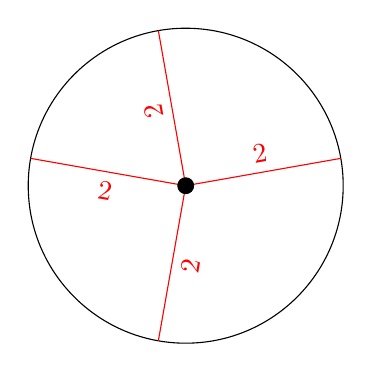
\begin{tikzpicture}
        \draw (0,0) circle (2);
        \draw[red] (0,0) -- node[midway,rotate=10,above] {$\qty{2}{\centi\metre}$} ({2*cos(10)},{2*sin(10});
        \draw[red] (0,0) -- node[midway,rotate=100,above] {$\qty{2}{\centi\metre}$} ({2*cos(100)},{2*sin(100});
        \draw[red] (0,0) -- node[midway,rotate=-10,below] {$\qty{2}{\centi\metre}$} ({2*cos(170)},{2*sin(170});
        \draw[red] (0,0) -- node[midway,rotate=80,below] {$\qty{2}{\centi\metre}$} ({2*cos(260)},{2*sin(260});
        \draw[black,fill=black] (0,0) circle (0.1);
    \end{tikzpicture}
\end{center}
}

\vocabulaire{Le \emph{diamètre} d'un cercle est un segment qui relie 2 points du cercle et qui passe par le centre du cercle.}

\illustration{
\begin{center}
    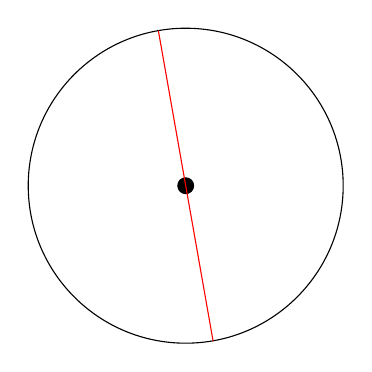
\begin{tikzpicture}
        \draw (0,0) circle (2);
        \draw[black,fill=black] (0,0) circle (0.1);
        \draw[red] ({2*cos(100)},{2*sin(100}) -- ({2*cos(280)},{2*sin(280});
    \end{tikzpicture}
\end{center}
}

\formule{$$\mbox{diamètre} = 2 \times \mbox{rayon}$$}

\definition{Une corde est un segment qui relie deux points du cercle.}

\illustration{
\begin{center}
    \begin{tikzpicture}
        \draw (0,0) circle (2);
        \coordinate (A) at ({2*cos(170)},{2*sin(170});
        \coordinate (B) at ({2*cos(90)},{2*sin(90});
        \coordinate (C) at ({2*cos(270)},{2*sin(270});
        \coordinate (D) at ({2*cos(330)},{2*sin(330});
        \draw[line width=1.2mm,red] (B) -- (A);
        \draw[line width=1.2mm,vert] (C) -- (D);
        \foreach \p/\x in {A/left,B/above,C/below,D/right} {
            \node[\x] at (\p) {$\p$};
        }
        \node at (5,1) {deux cordes : $[AB]$,$[CD]$};
    \end{tikzpicture}
\end{center}
}

\definition{Un arc de cercle est une portion du cercle qui relie deux points du cercle.}

\illustration{
\begin{center}
    \begin{tikzpicture}
        \draw (0,0) circle (2);
        \coordinate (A) at ({2*cos(170)},{2*sin(170});
        \coordinate (B) at ({2*cos(90)},{2*sin(90});
        \coordinate (C) at ({2*cos(270)},{2*sin(270});
        \coordinate (D) at ({2*cos(330)},{2*sin(330});
        \draw[line width=1.2mm,red] (A) arc (170:90:2);
        \draw[line width=1.2mm,vert!90!white] (C) arc (270:330:2);
        \foreach \p/\x in {A/left,B/above,C/below,D/right} {
            \node[\x] at (\p) {$\p$};
        }
        \draw (7.55,1.3) arc (160:20:0.35);
        \draw (8.4,1.3) arc (160:20:0.35);
        \node at (6,1) {deux arcs de cercle : $AB$,$CD$};
    \end{tikzpicture}
\end{center}
}

\formule{Le périmètre d'un cercle de rayon $r$ : $$P_{\mbox{cercle}} = \pi \times 2 \times r$$}

\remarque{Le nombre \pi{} est environ égal à \num{3,14}.}

\partie{Médiatrice}

\definition{La médiatrice d'un segment est la droite constituée de tous les points équidistants aux extrémités du segment.}

\illustration{
    \begin{center}
        \begin{tikzpicture}
            \draw (0,0) -- (2,0);
            \draw (1,2) -- (1,-1);
            \draw[black,fill=black] (0,0) circle (0.05);
            \draw[black,fill=black] (2,0) circle (0.05);
            \draw[red,fill=red] (1,1.3) circle (0.05);
            \draw[red] (0,0) -- (1,1.3) -- (2,0);
            \node[left] (A) at (0,0) {\small{$A$}};
            \node[right] (B) at (2,0) {\small{$B$}};
            \node[right,rouge] (M) at (1,1.3) {\small{$M$}};
        \end{tikzpicture}
    \end{center}
}

\construction{
\begin{center}
    \begin{tikzpicture}
        \draw (0,0) node[left]{$A$} -- (2,0) node[right]{$B$};
        \draw[vert] (1,-1.5) -- (1,2);
        \draw[black,fill=black] (0,0) circle (0.05);
        \draw[black,fill=black] (2,0) circle (0.05);
        \draw (1.3,0) arc (0:60:1.3);
        \draw (1.3,0) arc (0:-60:1.3);
        \draw (0.7,0) arc (180:120:1.3);
        \draw (0.7,0) arc (180:240:1.3);
    \end{tikzpicture}
\end{center}
\begin{itemize}
    \item Tracer le segment $[AB]$
    \item Prendre le compas, et choisir un écartement
    \item Placer la pointe du compas sur $A$ et tracer un arc de cercle
    \item Placer la pointe du compas sur $B$ et tracer un arc de cercle
    \item Relier les points d'intersections des arcs de cercle
\end{itemize}
}

\propriete{La médiatrice d'un segment coupe ce segment en son milieu et perpendiculairement.}

\illustration{
    \begin{center}
        \begin{tikzpicture}
            \draw (0,0) -- (2,0);
            \draw[vert] (1,2) -- (1,-1);
            \draw[black,fill=black] (0,0) circle (0.05);
            \draw[black,fill=black] (2,0) circle (0.05);
            \node[left] (A) at (0,0) {\small{$A$}};
            \node[right] (B) at (2,0) {\small{$B$}};
            \node[red] at ($(A)!0.35!(B)$) {\small{||}};
            \node[red] at ($(A)!0.65!(B)$) {\small{||}};
            \draw[red,fill=red] ($(A)!0.5!(B)$) rectangle +(0.2,0.2);
        \end{tikzpicture}
    \end{center}
}

\propriete{$M$ appartient à la médiatrice du segment $[AB]$ si et seulement si $MA=MB$.}



\end{document}